\begin{pastexam}[label={px:ncku-109-comm-ds-06}]{成大電通所 109 學年度 第 6 題}
（手算追蹤）

Consider a sequence of keys : 4, 7, 12, 15, 3, 5, 14, 18. Draw, \textbf{step by step} (showing
clearly the type of rotation used), the result of inserting these keys into an empty AVL tree.
(20 points)
\end{pastexam}

\begin{pastsoln}
照二元搜尋樹的規則插入，再從新節點往上找第一個平衡因子（左高減右高）變成 $\pm 2$ 的節點，依新節點在
它的哪一邊決定 LL、RR、LR、RL 四種旋轉（資結書第~10.2.3、10.2.4~節）。 旋轉只發生在插入 $12$ 和
$14$ 的時候。
\begin{enumerate}
\item 插入 $4$：只有根。
\item 插入 $7$：成為 $4$ 的右子節點，$4$ 的平衡因子 $-1$，不用轉。
\item 插入 $12$：成為 $7$ 的右子節點。 $4$ 的平衡因子 $-2$，新節點在 $4$ 的右子節點 $7$ 的右邊，是
\textbf{RR 型}，在 $4$ 做一次左旋，$7$ 成為根。
\item 插入 $15$：$15 > 7$、$15 > 12$，成為 $12$ 的右子節點。 $12$ 是 $-1$、$7$ 是 $-1$，不用轉。
\item 插入 $3$：成為 $4$ 的左子節點。 $4$ 是 $+1$、$7$ 是 $0$，不用轉。
\item 插入 $5$：$5 < 7$、$5 > 4$，成為 $4$ 的右子節點。 $4$ 是 $0$、$7$ 是 $+1$，不用轉。
\item 插入 $14$：$14 > 7$、$14 > 12$、$14 < 15$，成為 $15$ 的左子節點。 $15$ 是 $+1$，$12$ 是
$-2$，失衡。 新節點在 $12$ 的右子節點 $15$ 的\textbf{左}邊，是 \textbf{RL 型}：先在 $15$ 右旋、再在 $12$
左旋，$14$ 升上來，左右子節點是 $12$、$15$。 旋轉後這棵子樹高度回到插入前的 $1$（葉為 $0$），$7$ 不用
再調整。
\item 插入 $18$：$18 > 7, 14, 15$，成為 $15$ 的右子節點。 $15$ 是 $-1$、$14$ 是 $-1$、$7$ 是 $-1$，
不用轉。
\end{enumerate}

插入 12 以後各步驟的樹（標「失衡」的是旋轉前的狀態）：
\begin{center}
\begin{tabular}{ccc}
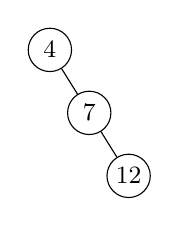
\begin{tikzpicture}[level distance=8mm,sibling distance=10mm,every node/.style={circle,draw,inner sep=0pt,minimum size=5.5mm,font=\small},baseline=(current bounding box.north)]
\node {4} child[missing] child {node {7} child[missing] child {node {12}}};
\end{tikzpicture}
&
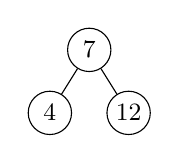
\begin{tikzpicture}[level distance=8mm,sibling distance=10mm,every node/.style={circle,draw,inner sep=0pt,minimum size=5.5mm,font=\small},baseline=(current bounding box.north)]
\node {7} child {node {4}} child {node {12}};
\end{tikzpicture}
&
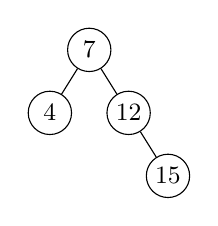
\begin{tikzpicture}[level distance=8mm,sibling distance=10mm,every node/.style={circle,draw,inner sep=0pt,minimum size=5.5mm,font=\small},baseline=(current bounding box.north)]
\node {7} child {node {4}} child {node {12} child[missing] child {node {15}}};
\end{tikzpicture}
\\[2pt]
插入 12，$4$ 失衡（RR） & 在 $4$ 左旋後 & 插入 15 \\[8pt]
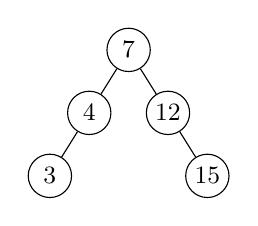
\begin{tikzpicture}[level distance=8mm,sibling distance=10mm,every node/.style={circle,draw,inner sep=0pt,minimum size=5.5mm,font=\small},baseline=(current bounding box.north)]
\node {7} child {node {4} child {node {3}} child[missing]} child {node {12} child[missing] child {node {15}}};
\end{tikzpicture}
&
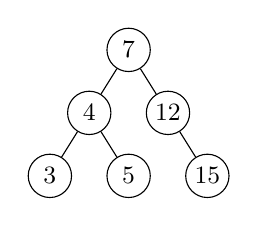
\begin{tikzpicture}[level distance=8mm,sibling distance=10mm,every node/.style={circle,draw,inner sep=0pt,minimum size=5.5mm,font=\small},baseline=(current bounding box.north)]
\node {7} child {node {4} child {node {3}} child {node {5}}} child {node {12} child[missing] child {node {15}}};
\end{tikzpicture}
&
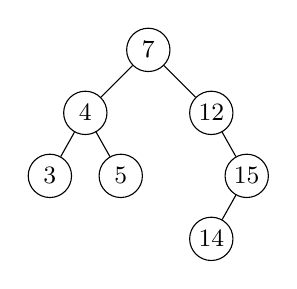
\begin{tikzpicture}[level distance=8mm,level 1/.style={sibling distance=16mm},level 2/.style={sibling distance=9mm},every node/.style={circle,draw,inner sep=0pt,minimum size=5.5mm,font=\small},baseline=(current bounding box.north)]
\node {7} child {node {4} child {node {3}} child {node {5}}} child {node {12} child[missing] child {node {15} child {node {14}} child[missing]}};
\end{tikzpicture}
\\[2pt]
插入 3 & 插入 5 & 插入 14，$12$ 失衡（RL） \\[8pt]
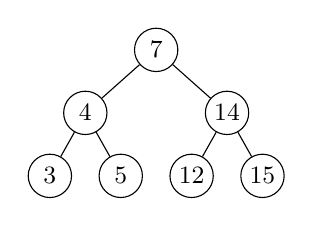
\begin{tikzpicture}[level distance=8mm,level 1/.style={sibling distance=18mm},level 2/.style={sibling distance=9mm},every node/.style={circle,draw,inner sep=0pt,minimum size=5.5mm,font=\small},baseline=(current bounding box.north)]
\node {7} child {node {4} child {node {3}} child {node {5}}} child {node {14} child {node {12}} child {node {15}}};
\end{tikzpicture}
&
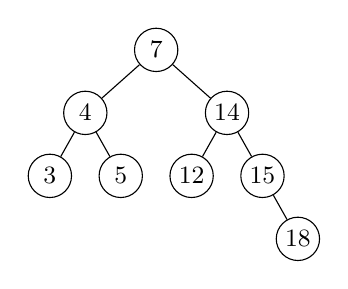
\begin{tikzpicture}[level distance=8mm,level 1/.style={sibling distance=18mm},level 2/.style={sibling distance=9mm},every node/.style={circle,draw,inner sep=0pt,minimum size=5.5mm,font=\small},baseline=(current bounding box.north)]
\node {7} child {node {4} child {node {3}} child {node {5}}} child {node {14} child {node {12}} child {node {15} child[missing] child {node {18}}}};
\end{tikzpicture}
& \\[2pt]
在 $15$ 右旋、$12$ 左旋後 & 插入 18（最後結果） & \
\end{tabular}
\end{center}
最後的 AVL 樹：根 $7$；左子樹 $4$（子節點 $3$、$5$）；右子樹 $14$（左 $12$，右 $15$，$15$ 的右子節點
$18$）。 中序是 $3, 4, 5, 7, 12, 14, 15, 18$，每個節點的平衡因子都在 $-1$ 到 $1$ 之間。
\end{pastsoln}
